\subsection{Taylor Series}
\subsubsection{Taylor/Maclaurin Series for a Function}
Suppose the function $f$ has derivatives of all orders on an interval containing the point $a$. The \textbf{Taylor series for $f$ centered at $a$} is

\begin{align}
    f(a) + f'(a)(x - a) + \frac{f''(a)}{2!}(x - a)^2 + \frac{f^{(3)}(a)}{3!}(x - a)^3 + \cdots & \\ = \sum ^{\infty} _{k = 0} \frac{f^{(k)}(a)}{k!}(x - a)^k.
\end{align}

A Taylor series centered at $0$ is called a \textbf{Maclaurin series}.

\subsubsection{Binomial Coefficients}
$\forall p, k \in \mathbb{R} \wedge k \geq 1$

\begin{equation}
    \binom{p}{k} = \frac{p(p - 1)(p - 2)\cdots(p - k + 1)}{k!}.
\end{equation}

With the special case of $\binom{p}{0} = 1$.

\subsubsection{Binomial Series}
$\forall p \in \mathbb{R} \wedge p \neq 0$, the Taylor series for $f(x) = (1 + x)^p$ centered at 0 is the \textbf{binomial series}

\begin{align}
    \sum _{k = 0} ^{\infty} x^k = \sum _{k = 0} ^{\infty} \frac{p(p - 1)(p - 2)\cdots(p - k + 1)}{k!} x^k & \\ = 1 + px +\frac{p(p - 1)(p - 2)}{3!}x^3 + \cdots
\end{align}

The series converges for $|x| < 1$ (and possibly at the endpoints, depending on $p$). If $p$ is a nonnegative integer, the series terminates and results in a polynomial of degree $p$.

\subsubsection{Convergence of Taylor Series}
Let $f$ have derivatives of all orders on an open interval $I$ containing $a$. The Taylor series for $f$ centered at $a$ converges to $f$ , for all $x$ in $I$, if and only if $\lim _{n \rightarrow \infty} R_n (x) = 0$, for all $x$ in $I$, where

\begin{equation}
    R_n(x) = \frac{f^{(n + 1)}(c)}{(n + 1)!}(x - a)^{n + 1}
\end{equation}

is the remainder at $x$ (with $c$ between $x$ and $a$).

\subsubsection{Taylor Series Functions}
\begin{center}
    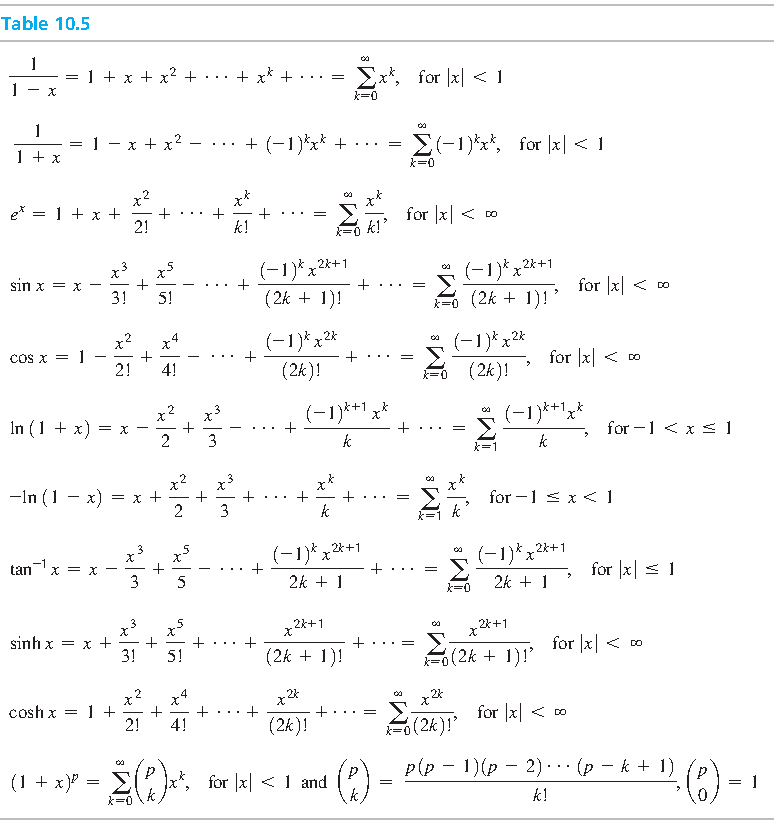
\includegraphics{assets/table.pdf}
\end{center}
